\paragraph{Sơ đồ tuần tự luồng cập nhật giao dịch thành công và Outbox}

Luồng nghiệp vụ này mô tả
nhánh IPN hợp lệ,
transaction còn ở trạng thái \texttt{pending}
và cổng thanh toán báo thanh toán thành công.
Dịch vụ thanh toán cập nhật transaction,
kích hoạt gói thuê bao VIP,
ghi sự kiện vào Outbox.
% trong cùng transaction lưu subscription,
% sau đó phát sự kiện miền qua NestJS CQRS EventBus.

\begin{figure}[H]
\centering
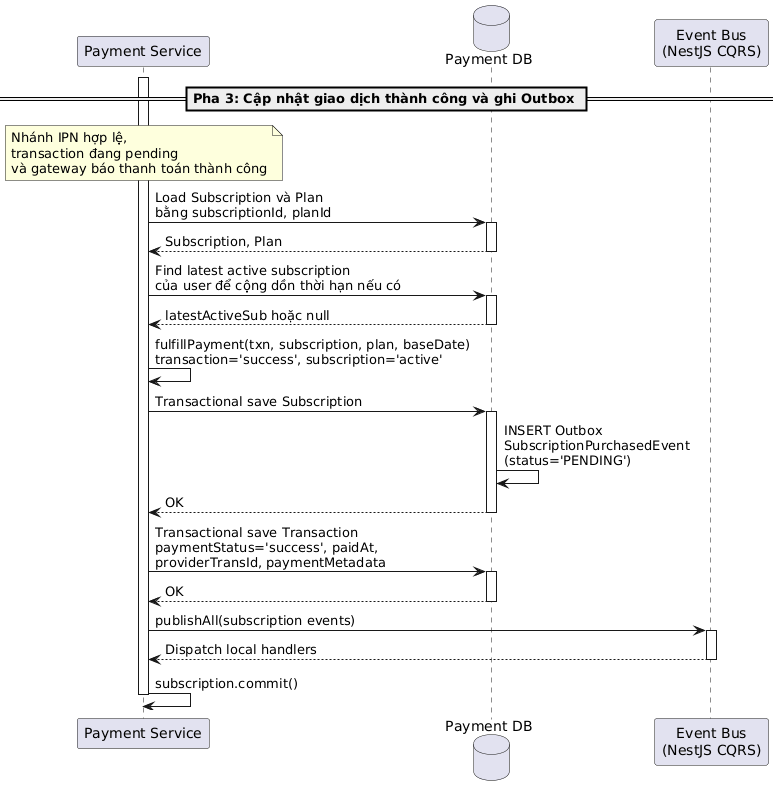
\includegraphics[width=0.65\textwidth]{contents/Sequence/UML-Sequence-PaymentSuccessUpdateOutbox.png}
\caption{Sơ đồ tuần tự luồng cập nhật giao dịch thành công và Outbox}
\end{figure}

\begin{table}[H]
\centering
\renewcommand{\arraystretch}{1.3}

\begin{tabular}{|l|l|p{5cm}|}
\hline
\textbf{Thành phần} & \textbf{Phân loại} & \textbf{Vai trò trong hệ thống} \\ \hline
Payment Service & Microservice & Xử lý nhánh thanh toán thành công, gọi domain service để cập nhật transaction và subscription. \\ \hline
Payment DB & Database & Lưu transaction, subscription và bản ghi Outbox. \\ \hline
Event Bus (NestJS CQRS) & Component & Phát domain event nội bộ cho các local handler sau khi lưu dữ liệu thành công. \\ \hline
\end{tabular}
\caption{Các thành phần tham gia luồng cập nhật giao dịch thành công và Outbox}
\end{table}

\subparagraph{Mô tả tổng quan}

\begin{itemize}

\item \textbf{Chuẩn bị thông tin kích hoạt:}
Dịch vụ thanh toán
lấy thông tin gói thuê bao VIP
và gói dịch vụ tương ứng dựa trên định danh giao dịch,
đồng thời tìm kiếm gói thuê bao VIP
đang hoạt động gần nhất của người dùng để cộng dồn thời hạn sử dụng nếu cần.

\item \textbf{Hoàn tất thanh toán:}
Dịch vụ cập nhật
trạng thái giao dịch thành công,
ghi nhận thời điểm thanh toán
và chuyển trạng thái gói thuê bao VIP thành đang hoạt động.

\item \textbf{Lưu sự kiện hệ thống:}
Dịch vụ ghi nhận sự kiện mua gói thuê bao VIP thành công
vào bảng sự kiện chờ gửi trong CSDL ở trạng thái chờ xử lý.

\item \textbf{Phát sự kiện nội bộ:}
Sau khi giao dịch được lưu thành công,
dịch vụ phát sự kiện nội bộ để các bộ phận khác
trong hệ thống tiếp tục xử lý và hoàn tất giao dịch.

\end{itemize}
